\documentclass[a4paper,11pt]{article}

% --- microtype ---
\usepackage[activate={true,nocompatibility},
            factor=1100,
            stretch=10,
            shrink=10]{microtype}  % improve general appearance
% activate - protrusion and expansion
% factor - add 10% to the protrusion amount (default is 1000)
% stretch / shrink - reduce stretchability/shrinkability (default is 20/20)

% \usepackage{palatino}  % ugly font [deprecated]
% \usepackage[sc]{mathpazo}  % same font but not deprecated package
\usepackage{pifont}  % special PostScript fonts (e.g. for xmark == ding{53})
% \usepackage[scaled=0.8]{luximono}  % fixed-width font that supports boldface (useful when typesetting source code)

% \usepackage{multicol}  % typeset text in multiple columns
\usepackage[titletoc]{appendix}  % prepend "Appendix" to chapter names
\usepackage{titlesec}  % help with section naming
% \usepackage{geometry}  % page dimensions, margins ...
% \usepackage{fancyhdr}  % customizing the headers and footers
% \usepackage{quotchap}  % fancy chapter heading pages
% \usepackage[parfill]{parskip}  % use no indentation and space between paragraphs
\usepackage{nicefrac}  % nicer fractions


% ----------------------------
% ----- Utility packages -----
\usepackage{empheq}  % for colorbox
\usepackage{mdframed}  % for box around figures

\usepackage{lipsum}
\usepackage{blindtext}

\usepackage{enumitem}  % much easier to make modifications to lists
% \usepackage{paralist}  % Improves enumerate and itemize. Also provides some compact environments

\usepackage{ifthen}  % used in \clearemptydoublepage
\usepackage{rotating}  % rotation tools, including rotated full-page floats
\usepackage{xparse}  % more flexible macros with more than one optional argument

% --- margin notes ---
\usepackage{marginnote}
\usepackage{mparhack}
\usepackage{marginfix}


% ------------------------------
% ----- Document structure -----
\usepackage{booktabs}  % for elegant tables
\usepackage[acronym,symbols,
            nomain,nogroupskip,nonumberlist,nopostdot,  % xindy,
            toc]{glossaries}
\usepackage{glossary-longbooktabs}
  \newglossary[slg]{symbolslist}{syi}{syg}{Symbolslist}
  \makeglossaries
% \usepackage{makeidx}  % standard LaTeX package for creating indexes
% xindy - more flexible than makeindex (sudo apt install xindy)
\usepackage{subfiles}


% ------------------------
% ----- Bibliography -----
\usepackage{csquotes}
\usepackage[english]{babel}  % set default language to English
% \usepackage[backend=biber,
%             bibstyle=authoryear,
%             citestyle=authoryear,%apa,
%             % natbib=true,
%             hyperref=true,
%             isbn=true,
%             doi=true,
%             url=true,
%             eprint=true]{biblatex}
% \DeclareLanguageMapping{english}{english-apa}

% --- apacite ---
\usepackage[natbibapa]{apacite}
  \bibliographystyle{apacite}
\usepackage[hyphens,spaces]{url}

% --- plain natbib ---
% \usepackage[round, sort]{natbib}
% \bibliographystyle{plainnat}

\usepackage[nottoc,numbib]{tocbibind}  % add bibliography & listings to ToC

% ------------------
% ----- Tables -----
\usepackage{tabularx}
\usepackage{tabu}  % tables
% \usepackage{colortbl}  % add color to LaTeX tables
% \usepackage{multirow}  % tabular cells spanning multiple rows
% \usepackage{dcolumn}  % columns of different types and alignment


% ----------------
% ----- Math -----

% --- AMS facilities ---
\usepackage{amsmath}
\usepackage{amsthm}
\usepackage{amsfonts}
\usepackage{amssymb}

\usepackage{mathtools}
\usepackage[retainorgcmds]{IEEEtrantools}  % sophisticated equation arrays
% \usepackage{yhmath}  % extended maths fonts for LaTeX
% \usepackage{commath}  % math delimiters of auto computed size
% \usepackage{comment}
% \usepackage{kbordermatrix}  % add column and row labels to matrices
\usepackage{physics}  % \bra, \ket, \expval, \mel ...
                      % & \abs, \norm, \var, \tr, \Tr ...


% -------------------------------
% ----- Graphics and floats -----
\usepackage{float}  % improved interface for floating objects
\usepackage{caption}
\usepackage{subcaption}  % to use subfigures
\usepackage{graphicx}  % enhanced support for graphics
  \graphicspath{{figures/}{../figures/}}  % in gereral {{subdir1/}...{subdirn/}}

% \usepackage{tikz}
% \usepackage{pgfplots}  % uses PGF to draw professionally looking charts and plots

% -----------------
% ----- Color -----
\usepackage[dvipsnames]{xcolor}  % color (+ in math mode)
% pre-defined colors: https://en.wikibooks.org/wiki/LaTeX/Colors#Predefined_colors

% --- my colors ---
\definecolor{tumblue}{HTML}{0065BD}
\definecolor{darkblue}{HTML}{001473}
\definecolor{darkgray}{RGB}{100, 100, 100}
\definecolor{ddarkgray}{RGB}{66, 66, 66}
\definecolor{gray}{rgb}{0.5,0.5,0.5}
\definecolor{orange}{rgb}{1.0,0.3,0.01}
\definecolor{violet}{rgb}{0.4,0.0,0.6}
\definecolor{yellow}{rgb}{1.0,0.7,0.0}
\definecolor{boxc}{rgb}{1.0, 1.0, .9}
\definecolor{mygreen}{rgb}{0, 0.75, 0.18}

% --- hyperref colors ---
\def\linkcolor{tumblue}
\def\urlcolor{darkblue}
\def\citecolor{darkblue}


% -----------------------
% ----- Source code -----
% \usepackage{listings} % (optional - alternative)
% \usepackage[newfloat]{minted} % (recommended)
% Set global Minted options
% \setminted{linenos, autogobble, frame=lines, framesep=2mm}
%%% Inline C++ (optional)
% \newcommand{\incpp}[1]{\mintinline{c++}{#1}}
% \newenvironment{code}{\captionsetup{type=listing}}{}
% \SetupFloatingEnvironment{listing}{name=Source Code}


% -----------------------------------
% ----- Algorithms (pseudocode) -----
\usepackage{algorithmicx}
\usepackage{algpseudocode}
  \algrenewcommand{\algorithmiccomment}[1]{\hfill$\rightarrow$ #1}  % normal arrow comments


% --------------------
% ----- Hyperref -----
\usepackage[linktocpage,
            colorlinks=true,
            bookmarksnumbered=true]{hyperref}

% set links colors
\hypersetup{
  linkcolor=\linkcolor,%
  urlcolor=\urlcolor,%
  citecolor=\citecolor
}

% disable the coloring of the links when printing
\usepackage[ocgcolorlinks]{ocgx2}[2017/03/30]

% PDF metadata
% \hypersetup{
%   pdftitle={\metatitle},%
%   pdfauthor={\metaauthor},%
%   pdfkeywords={\metakeywords},%
%   pdfsubject={\metasubject}
% }

% ----------------------------------------------------------------------------------
% ----- Utilities that must go after other packages (`hyperref`, `xcolor` ...) -----
\usepackage{bookmark}  % better bookmark handling (loads hyperref)
\usepackage{hyperxmp}  % create XMP Metadata (uses the values from hyperref)
\usepackage{xspace}  % define commands that do not eat spaces
% \usepackage{thumbpdf}  % make thumbnails
\usepackage{todonotes}
% \usepackage{fancyvrb}  % highly customisable verbatim


% -----------------------------
% ----- General shortcuts -----
% \renewcommand{\sf}[1]{\textsf{#1}}
% \renewcommand{\tt}[1]{\texttt{#1}}
% \renewcommand{\bf}[1]{\textbf{#1}}
% \renewcommand{\sl}[1]{\textsl{#1}}
% \renewcommand{\sc}[1]{\textsc{#1}}
% \newcommand{\e}[1]{\emph{#1}}

\renewcommand{\u}[1]{\underline{#1}}

\newcommand{\gooditem}{\item[\checkmark]}
\newcommand{\baditem}{\item[\ding{53}]}
\newcommand{\good}{\textbf{\color{green}[\checkmark]}}
\newcommand{\bad}{\textbf{\color{red}[\ding{53}]}}


% ----------------------------
% ----- General commands -----
\newcommand{\commentinline}[1]{\color{darkgray}\left[\text{#1}\right]\color{black}}
\newcommand{\commentii}[2]{\color{darkgray}\left[\begin{array}{c}\text{#1}\\ \text{#2}\end{array}\right]\color{black}}


% --------------------------------------
% ----- Document layout/formatting -----

% page clearing
\newcommand{\clearemptydoublepage}{%
  \ifthenelse{\boolean{@twoside}}{\newpage{\pagestyle{empty}\cleardoublepage}}%
  {\clearpage}}

% comment that appears on the border
\newcommand{\mcomment}[1]{\marginpar{\raggedright \noindent {\textsl{#1}}}}


% insert figure (fname, caption for ToC, caption, label, width as fraction of \textwidth)
\newcommand{\insertfig}[5]{
	\begin{figure}[htbp]
		\begin{center}
			\includegraphics[width=#5\textwidth]{#1}  % width, height, scale, angle ...
		\end{center}
		\vspace{-0.4cm}
		\caption[#2]{#3}
		\label{fig:#4}
	\end{figure}
}

% --- color box ---
\newlength\mytemplen
\newsavebox\mytempbox

\makeatletter

\newcommand\mybox{%
    \@ifnextchar[%]
       {\@mybox}%
       {\@mybox[0pt]}}

\def\@mybox[#1]{%
    \@ifnextchar[%]
       {\@@mybox[#1]}%
       {\@@mybox[#1][0pt]}}

\def\@@mybox[#1][#2]#3{
    \sbox\mytempbox{#3}%
    \mytemplen\ht\mytempbox
    \advance\mytemplen #1\relax
    \ht\mytempbox\mytemplen
    \mytemplen\dp\mytempbox
    \advance\mytemplen #2\relax
    \dp\mytempbox\mytemplen
    \colorbox{boxc}{\hspace{0em}\usebox{\mytempbox}\hspace{0em}}}

\makeatother


% ----------------------
% ----- References -----

% suffixes are consistent with:
% https://en.wikibooks.org/wiki/LaTeX/Labels_and_Cross-referencing
\newcommand{\refch}[1]{chapter \ref{ch:#1}}
\newcommand{\refsec}[1]{section \ref{sec:#1}}
\newcommand{\refsubsec}[1]{subsection \ref{subsec:#1}}
\newcommand{\reffig}[1]{figure \ref{fig:#1}}
\newcommand{\reftab}[1]{table \ref{tab:#1}}
\renewcommand{\refeq}[1]{equation \eqref{eq:#1}}
\newcommand{\reflst}[1]{listing \ref{lst:#1}}  % code listing
\newcommand{\refitm}[1]{\ref{itm:#1}}  % enumerated list item
\newcommand{\refalg}[1]{algorithm \ref{alg:#1}}
\newcommand{\refapp}[1]{appendix \ref{app:#1}}

\newcommand{\refCh}[1]{Chapter \ref{ch:#1}}
\newcommand{\refSec}[1]{Section \ref{sec:#1}}
\newcommand{\refSubsec}[1]{Subsection \ref{subsec:#1}}
\newcommand{\refFig}[1]{Figure \ref{fig:#1}}
\newcommand{\refTab}[1]{Table \ref{tab:#1}}
\newcommand{\refEq}[1]{Equation \eqref{eq:#1}}
\newcommand{\refLst}[1]{Listing \ref{lst:#1}}  % code listing

\newcommand{\refAlg}[1]{Algorithm \ref{alg:#1}}
\newcommand{\refApp}[1]{Appendix \ref{app:#1}}


% --------------------------------------------
% ----- Theorems environments & counters -----
% \newtheorem{theorem}{Theorem}[chapter]
% \newtheorem{lemma}[theorem]{Lemma}
% \newtheorem{corollary}[theorem]{Corollary}
% \newtheorem{remark}[theorem]{Remark}
% \newtheorem{definition}[theorem]{Definition}
% \newtheorem{equat}[theorem]{Equation}
% \newtheorem{example}[theorem]{Example}
% \newtheorem{algorithm}[theorem]{Algorithm}


% ----------------------
% ----- Math stuff -----

% --- general shortcuts ---
\renewcommand{\l}{\left}
\renewcommand{\r}{\right}
\renewcommand{\o}[1]{\overline{#1}}
\newcommand{\ub}[2]{\underbrace{#1}_{#2}}
\newcommand{\ob}[2]{\overbrace{#1}_{#2}}

% --- fonts & boldness ---
\newcommand{\bs}[1]{\boldsymbol{#1}}
\newcommand{\mr}[1]{\mathrm{#1}}
\newcommand{\mb}[1]{\mathbf{#1}}
\newcommand{\mc}[1]{\mathcal{#1}}
\newcommand{\mf}[1]{\mathfrak{#1}}

% --- shortcuts to common quantities ---
\newcommand{\half}{\frac{1}{2}}

% --- shortcuts for delimiters with correct auto-size ---
% (names are consistent with `matrix` environment)
\newcommand{\p}[1]{ \left( #1 \right) }
\renewcommand{\b}[1]{ \left[ #1 \right] }
\newcommand{\B}[1]{ \left\{ #1 \right\} }
\renewcommand{\v}[1]{ \left| #1 \right| }
\newcommand{\V}[1]{ \left\| #1 \right\| }

% --- general math ---
\DeclareMathOperator*{\argmax}{arg\,max}
\DeclareMathOperator*{\argmin}{arg\,min}
\DeclareMathOperator{\const}{const}
\DeclareMathOperator{\e}{e}  % exp
\newcommand{\ind}[1]{\mathbbm{1}_{\left\lbrace #1 \right\rbrace}}

% better defaults
\renewcommand{\epsilon}{\varepsilon}
\newcommand{\eps}{\epsilon}
\renewcommand{\kappa}{\varkappa}
\renewcommand{\geq}{\geqslant}
\renewcommand{\leq}{\leqslant}

% spaces
\newcommand{\N}{\mathbb{N}}
\newcommand{\Z}{\mathbb{Z}}
\newcommand{\Q}{\mathbb{Q}}
\newcommand{\R}{\mathbb{R}}
\newcommand{\C}{\mathbb{C}}

% \DeclarePairedDelimiter{\abs}{\lvert}{\rvert}
\let\abs\relax\newcommand{\abs}[1]{\left\lvert #1 \right\rvert}

% --- linear algebra ---
\let\tr\relax\DeclareMathOperator{\tr}{tr}
\let\Tr\relax\DeclareMathOperator{\Tr}{Tr}

% \newcommand{\norm}[1]{\left\lVert #1 \right\rVert}
\newcommand{\vecii}[2]{\begin{array}[h]{c} #1 \\ #2	\end{array}}
\newcommand{\veciii}[3]{\begin{array}[h]{c} #1 \\ #2 \\ #3	\end{array}}
\newcommand{\veciv}[4]{\begin{array}[h]{c} #1 \\ #2 \\ #3 \\ #4	\end{array}}

\newcommand{\matii}[4]{\begin{array}[h]{ccc} #1 & #2 \\ #3 & #4 \end{array}}
\newcommand{\matiii}[9]{\begin{array}[h]{ccc} #1 & #2 & #3 \\ #4 & #5 & #6 \\ #7 & #8 & #9	\end{array}}

% --- calculus ---
\newcommand{\evalat}[1]{\biggr\rvert _{#1}}
% \newcommand{\pd}[2]{ \frac{\partial #1}{\partial #2} }  % partial derivative
\DeclareDocumentCommand{\pd}{ O{} O{} m }{\frac{\partial^{#2}#1}{\partial#3^{#2}}}  % partial derivative

\renewcommand{\d}{\mathrm{d}}  % upright "d" for differential
\newcommand{\ud}{\,\mathrm{d}}  % correct spacing for differential in integral

% --- probability theory ---
\let\var\relax\DeclareMathOperator{\var}{var}
\DeclareMathOperator{\med}{med}

\newcommand{\E}{\mathbb{E}}
\renewcommand{\P}[1]{\mathbb{P}\left\lbrace #1 \right\rbrace}
\renewcommand{\Pr}[1]{\operatorname{Pr}\left\lbrace #1 \right\rbrace}
\newcommand{\pr}[1]{p\left( #1 \right)}

% --- information theory ---
\newcommand{\KL}[2]{\operatorname{KL}(#1 \parallel #2)}
\newcommand{\DKL}[2]{D_{\operatorname{KL}}(#1 \parallel #2)}


% ----------------
% ----- Misc -----

% --- some abreviations ---
\newcommand{\Reg}{$^{\textregistered}$}
\newcommand{\reg}{$^{\textregistered}$ }
\newcommand{\Tm}{\texttrademark}
\newcommand{\tm}{\texttrademark~}
\newcommand{\bsl}{$\backslash$}

% # General
% ## LaTeX shortcuts
\renewcommand{\l}{\left}
\renewcommand{\r}{\right}
\renewcommand{\o}[1]{\overline{#1}}
\newcommand{\ub}[2]{\underbrace{#1}_{#2}}
\newcommand{\ob}[2]{\overbrace{#1}_{#2}}
\newcommand{\half}{\frac{1}{2}}

% ## Better LaTeX defaults
\renewcommand{\epsilon}{\varepsilon}
\newcommand{\eps}{\epsilon}
\renewcommand{\kappa}{\varkappa}
\renewcommand{\geq}{\geqslant}
\renewcommand{\leq}{\leqslant}

% ## Math delimiters with correct auto-size
% * names are consistent with `matrix` environment prefixes
\newcommand{\p}[1]{ \left( #1 \right) }
\renewcommand{\b}[1]{ \left\lbrack #1 \right\rbrack }
\newcommand{\B}[1]{ \left\lbrace #1 \right\rbrace }
\renewcommand{\v}[1]{ \left\lvert #1 \right\rvert }
\newcommand{\V}[1]{ \left\| #1 \right\| }

% ## New delimiters
\newcommand{\llbracket}{[\![}
\newcommand{\rrbracket}{]\!]}

% ## Comments within math derivations
\newcommand{\commentinline}[1]{\color{darkgray}\left[\text{#1}\right]\color{black}}
\newcommand{\commentii}[2]{\color{darkgray}\left[\begin{array}{c}\text{#1}\\\text{#2}\end{array}\right]\color{black}}


% # By areas of science
% ## Elementary math
\DeclareMathOperator*{\argmax}{arg\,max}
\DeclareMathOperator*{\argmin}{arg\,min}
\DeclareMathOperator{\const}{const}
\DeclareMathOperator{\e}{e}  % exp
\newcommand{\ind}[1]{\mathbbm{1}_{\left\lbrace #1 \right\rbrace}}
% \newcommand{\Id}{\ensuremath{\mathds{1}}}

% \DeclarePairedDelimiter{\abs}{\lvert}{\rvert}
\let\abs\relax\newcommand{\abs}[1]{\left\lvert #1 \right\rvert}

\newcommand{\N}{\ensuremath{\mathbb{N}}}
\newcommand{\Z}{\ensuremath{\mathbb{Z}}}
\newcommand{\Q}{\ensuremath{\mathbb{Q}}}
\newcommand{\R}{\ensuremath{\mathbb{R}}}
\newcommand{\C}{\ensuremath{\mathbb{C}}}

% ## Linear algebra
\let\tr\relax\DeclareMathOperator{\tr}{tr}
\let\Tr\relax\DeclareMathOperator{\Tr}{Tr}
\DeclareMathOperator{\diag}{diag}

\let\norm\relax\newcommand{\norm}[1]{\left\lVert #1 \right\rVert}
\newcommand{\vecii}[2]{\begin{array}[h]{c} #1 \\ #2	\end{array}}
\newcommand{\veciii}[3]{\begin{array}[h]{c} #1 \\ #2 \\ #3 \end{array}}
\newcommand{\veciv}[4]{\begin{array}[h]{c} #1 \\ #2 \\ #3 \\ #4	\end{array}}

\newcommand{\matii}[4]{\begin{array}[h]{ccc} #1 & #2 \\ #3 & #4 \end{array}}
\newcommand{\matiii}[9]{\begin{array}[h]{ccc} #1 & #2 & #3 \\ #4 & #5 & #6 \\ #7 & #8 & #9 \end{array}}

% ## Calculus
\newcommand{\evalat}[2]{\left. #1 \right\rvert_{#2}}
% \newcommand{\pd}[2]{ \frac{\partial #1}{\partial #2} }  % partial derivative
\DeclareDocumentCommand{\pd}{ O{} O{} m }{\frac{\partial^{#2}#1}{\partial#3^{#2}}}  % partial derivative

% \newcommand{\pd}{\partial}  % partial differential
\renewcommand{\d}{\mathrm{d}}  % upright "d" for differential
\newcommand{\ud}{\,\mathrm{d}}  % correct spacing for differential in integral

% ## Probability theory
\let\var\relax\DeclareMathOperator{\var}{var}
\DeclareMathOperator{\med}{med}

\newcommand{\E}{\mathbb{E}}
\renewcommand{\P}[1]{\mathbb{P}\left\lbrace #1 \right\rbrace}
\renewcommand{\Pr}[1]{\operatorname{Pr}\left\lbrace #1 \right\rbrace}
\newcommand{\pr}[1]{p\left( #1 \right)}

% ## Information theory
\newcommand{\KL}[2]{\operatorname{KL}(#1 \parallel #2)}
\newcommand{\DKL}[2]{D_{\operatorname{KL}}(#1 \parallel #2)}

% ## Computer Science
% \newcommand{\Poly}{\ensuremath{\mathds{P}}}
%\newcommand{\O}{\ensuremath{\mathcal{O}}}
% \renewcommand{\O}{\ensuremath{\mathcal{O}}}

% ## Semantic formatting
\newcommand{\cmd}[1]{\texttt{#1}}
% # Semantic font styles for math quantities
% TODO: scalar, vector, matrix, tensor, dist
% The default optimizer is \texttt{RMSProp} \textsc?
% data-spaces \mathcal{X}, \mathcal{Y}; data \mathcal{D}
% \newcommand{\Pth}{\mathrm{P}_{\theta}}
% \newcommand{\Pz}{\mathrm{P}_z}



% ## title
\title{Title}
\author{
  Author\thanks{thanks}\\
  \texttt{email1}
  \and
  Author2\thanks{thanks}\\
  \texttt{email2}
}
\date{}

% ## bibliography using `biblatex`
% \addbibresource{bibliography/bib.bib}

\begin{document}
  \maketitle

  % ## common
  \tableofcontents
  % \listoftables
  % \listoffigures
  % {\let\cleardoublepage\clearpage \chapter{Chapter}\label{ch:label}}
  % \listoftodos

  \section{Essential} \label{sec:label}
  % ## annotation
  \todo{\textbackslash todo}
  \marginpar{\textbackslash marginpar}
  \mcomment{\small \textbackslash mcomment}

  % ## equation
  \begin{IEEEeqnarray}{rCl}
    \binom{n}{k}
      &=& \frac{n!}{k!(n-k)!} \label{eq:label1}
      \\[0.5em]
      &=& \frac{1}{2\pi i}\oint\limits_{\Gamma} \frac{ (1+z)^n }{z^{k+1}} \ud z
      \label{eq:label2}
  \end{IEEEeqnarray}

  % ## table
  \renewcommand\arraystretch{1.25}
  % break lines within cells with fixed-width columns using `array`

  \begin{table}[h]
    \centering
    \caption{Caption}
    \label{tab:label}
    \begin{tabular}{cc}
      \toprule
      A & \R \footnotemark \\
      \midrule
      a & b \\
      c & d \\
      \midrule
      e & f \\
      g & h \\
      \bottomrule
    \end{tabular}
    % OR caption & label here ...
  \end{table}

  \footnotetext{footnotemark--footnotetext}

  % ## figure
  \insertfig{death-star}{Caption for ToC}{Caption}{label}{0.2}  % `fig:label`

  % ## cite
  \noindent TensorFlow\footnote{footnote} \citep{tf}, \citet{tf}.\\
  Section \ref{sec:label} on a page \pageref{sec:label},
  table \ref{tab:label}, figure \ref{fig:label},
  equations \eqref{eq:label1} and \eqref{eq:label2}.


  \section{Other CO\texorpdfstring{\textsubscript{2}}{2}}
  \subsection*{Subfigures}
  % use `minipage` for individual figures numbering

  \begin{figure}[htb]
    \centering
    %
    \begin{subfigure}[b]{.475\textwidth}
      \frame{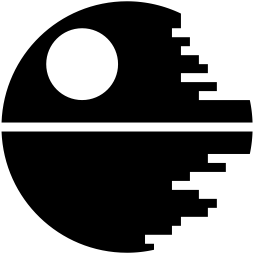
\includegraphics[width=\textwidth]{death-star}}
      \caption{Caption 1}  % or \subcaption
      \label{fig:1}
    \end{subfigure}
    \hfill
    \begin{subfigure}[b]{.475\textwidth}
      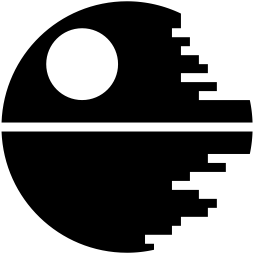
\includegraphics[width=\textwidth]{death-star}
      \caption{Caption 2}
      \label{fig:2}
    \end{subfigure}
    %
    \begin{subfigure}[b]{.3\textwidth}
      \frame{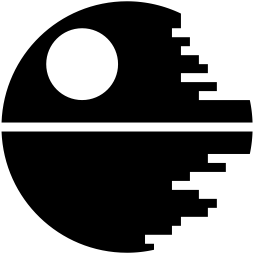
\includegraphics[width=\textwidth]{death-star}}
      \caption{Caption 3}
      \label{fig:3}
    \end{subfigure}
    \hfill
    \begin{subfigure}[b]{.3\textwidth}
      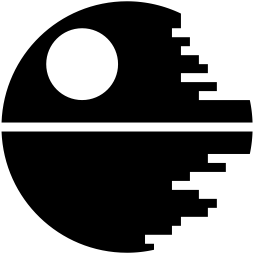
\includegraphics[width=\textwidth]{death-star}
      \caption{Caption 4}
      \label{fig:4}
    \end{subfigure}
    \hfill
    \begin{subfigure}[b]{.3\textwidth}
      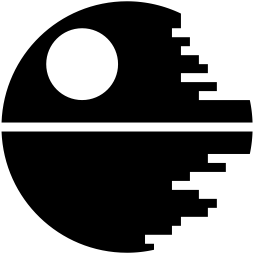
\includegraphics[width=\textwidth]{death-star}
      \caption{Caption 5}
      \label{fig:5}
    \end{subfigure}
    %
    \caption{The caption. \emph{Top}: top. \emph{Bottom}: bottom.}
    \label{fig:subfigures}
  \end{figure}

  \subsection*{Proof}
    \begin{proof}[\unskip\nopunct]
      The proof is easy and is left to a reader.
    \end{proof}

  \subsection*{Test math}
    \begin{gather*}
      {\textstyle \underset{\mu}{\sum} \; \sum_{\mu}} \; \R^{n\times m}\; \bra{\frac{\Psi}{1}} \; \ket{\frac{\Psi}{1}} \;
      \braket{\frac{\Psi}{1}} \;
      \matrixelement{n}{\prod_k U_k}{\frac{x}{1}} \;
      \mel{n}{\prod_k U_k}{\frac{x}{1}} \\
      \text{Normal}(\mathrm{x} \mid \mu, \sigma^2 ) \\
      \textnormal{Normal}(\mathrm{x} \mid \mu, \sigma^2 ) \\
      \mathrm{Normal}(\mathrm{x} \mid \mu, \sigma^2 ) \\
      \mathcal{N}(\mathrm{x} \mid \mu, \sigma^2 ) \\
      \sum_{\mathclap{n=-\infty}}^{+\infty} f(x) \geqslant \geq \ge \med X \\
      \eps + \e^{-\frac{(x-2)^2}{2\sigma ^2}} + \const{} \\
      \dot{a} \epsilon \phi \varphi \\
      \not\propto \not\subset \not\in \notin \\
      \equiv \doteq \approx \subset \supset \ni \mid \parallel \neq \ne \\
      \Tr A = \tr A = \var X = \KL{P}{Q} = \DKL{P}{Q} \\
      \star \ast \circ \bullet \oplus \otimes \odot \dagger \ddagger \text{\dag \ddag} \\
      \bigoplus \bigotimes \bigodot \bigcup \bigcap \\
      \leftarrow \gets \rightarrow \to \mapsto
      \Leftarrow \Rightarrow \Longleftrightarrow \iff \overrightarrow{AB} \rightrightarrows \\
      []\lbrack \rbrack \lbrace \rbrace \langle \rangle
      | \vert \| \Vert \lfloor \rfloor \arrowvert \Arrowvert \\
      \ell \emptyset \Re \Im \bot \top \angle \Box \\
      \thicksim \thickapprox \backsim \varpropto \risingdotseq \fallingdotseq \\
      \hbar \square \blacksquare \bigstar \varnothing
    \end{gather*}

    \begin{equation}
      \begin{Vmatrix}
        1 & 2 \\
        3 & 4
      \end{Vmatrix}
      =
      \abs{\oint_{A}^{B} f(z) \ud z}
      =
      \frac{\d u}{\d x}
      = \mathcal{F}\mathfrak{F}
      = \frac{\displaystyle \sum a_{ij} }{\displaystyle \sum b_{ij} }
      = \sum_{\mathclap{\text{big long thing}}} a_k
      = \frac{\displaystyle \P{\frac{X}{\E X} \leq \epsilon}}
             {\displaystyle \Pr{\mathrm{Poisson}(\lambda=3) > 5}}
    \end{equation}

    \begin{equation}
      \pd \cdot \pdd{x} \cdot \pdd[f]{x} \cdot \pdd[f][3]{x}
      \cdot \evalat{\pdd{x}\frac{x^2+1}{x^3+1}}{x=0}
      =
      \d \cdot \dd{x} \cdot \dd[f]{x} \cdot \dd[f][3]{x}
      \cdot \evalat{\dd{x}\frac{x^2+1}{x^3+1}}{x=0}
    \end{equation}

    \begin{equation}
      \o{a} \enskip
      A \stackrel{*}{\approx} B \enskip
      \sum_{\substack{0<i<n \\ j \neq i}}f(i) \enskip
      \sqrt[3]{P(x)+Q(x)} \enskip
      \frac{3}{8} \tfrac{3}{8} \dfrac{3}{8} 3/8 \enskip
      x=x\phantom{=}x\mathbin{=}x
    \end{equation}

  \subsection*{Math fonts}
    \begin{gather}
      \mathrm{ABCDEFabcdef} \tag{mathrm} \\
      \mathbf{ABCDEFabcdef} \tag{mathbf} \\
      \mathsf{ABCDEFabcdef} \tag{mathsf} \\
      \mathtt{ABCDEFabcdef} \tag{mathtt} \\
      \mathit{ABCDEFabcdef} \tag{mathit} \\
      \mathcal{ABCDEFabcdef} \tag{mathcal} \\
      \mathnormal{ABCDEFabcdef} \tag{mathnormal}
      \\[0.5em]
      \boldsymbol{ABCabc \Gamma\Omega\Xi \gamma\omega\xi } \tag{boldsymbol} \\
      \mathscr{ABCDEFabcdef} \tag{mathscr} \\
      \mathfrak{ABCDEFabcdef} \tag{mathfrak} \\
      \mathbb{ABCDEFabcdef12345} \tag{mathbb} \\
      \mathbbm{ABCDEFabcdef12345} \tag{mathbbm}
    \end{gather}

  \subsection*{Text fonts}
    \noindent
    \textrm{ABCDEFabcdef}  % RoMan
    \textsf{ABCDEFabcdef}  % Sans seriF
    \texttt{ABCDEFabcdef}  % Type wriTer
    \\[0.5em]
    \textmd{ABCDEFabcdef}  % MeDium
    \textbf{ABCDEFabcdef}  % Bold Face
    \\[0.5em]
    \textup{ABCDEFabcdef}  % UPright
    \textit{ABCDEFabcdef}  % ITalic
    \textsl{ABCDEFabcdef}  % SLanted
    \textsc{ABCDEFabcdef}  % Small Caps
    \\[0.5em]
    \textnormal{ABCDEFabcdef}  % document font
    \emph{ABCDEFabcdef}    % EMPHasize

  \subsection*{General formatting}
    \begin{itemize}[noitemsep]
      \item x \hspace{\stretch{1}} y \hspace{\stretch{1}} z \hspace*{\stretch{1}}
      \item ``quote''
      \item Ph.~D.
      \item Ph.\ D.
      \item Ph. D.
      \item A. B
      \item A\@. B
      \item \verb*+yo wazup+
    \end{itemize}

  % # Bibliography
  \newpage
  % ## bibliography using `biblatex`
  % \setlength\bibitemsep{1.5\itemsep}
  % \printbibliography

  % ## bibliography using `natbib`
  \setlength\bibsep{1.5\itemsep}
  \renewcommand{\bibname}{Bibliography}
  \bibliography{bibliography/bib}

\end{document}
